Los cinco bloques principales en los que se divide la planificación y que recoge el cuadro 2.1 son los siguientes:

\begin{itemize}
    \item Desarrollo incial: recopilación de información e implementación inicial.
    \item Entrenamiento: implementación del proceso de entrenamiento de modelos,entrenamiento y recogida de resultados.
    \item Implementación de la interfaz.
    \item Evaluación final: análisis y comparación de resultados.
    \item Documentación: redacción de la memoria y de la pertinente documentación del código.
\end{itemize}


En esta planificación se asumía que, una vez entrenados los modelos, la evaluación consistiría principalmente en ejecutar las métricas definidas, probar los modelos generados y valorar los resultados obtenidos. Sin embargo, durante el desarrollo del proyecto fueron surgiendo varios problemas que modificaron el desarrollo previsto. Finalmente la ejecución del proyecto se puede ver en el cronograma de la Figura 2.1, las incidencias que han causado los retrasos en la planificación son las enumeradas a continuación.

\begin{figure}[H]
    \centering
    \makebox[\textwidth][c]{%
        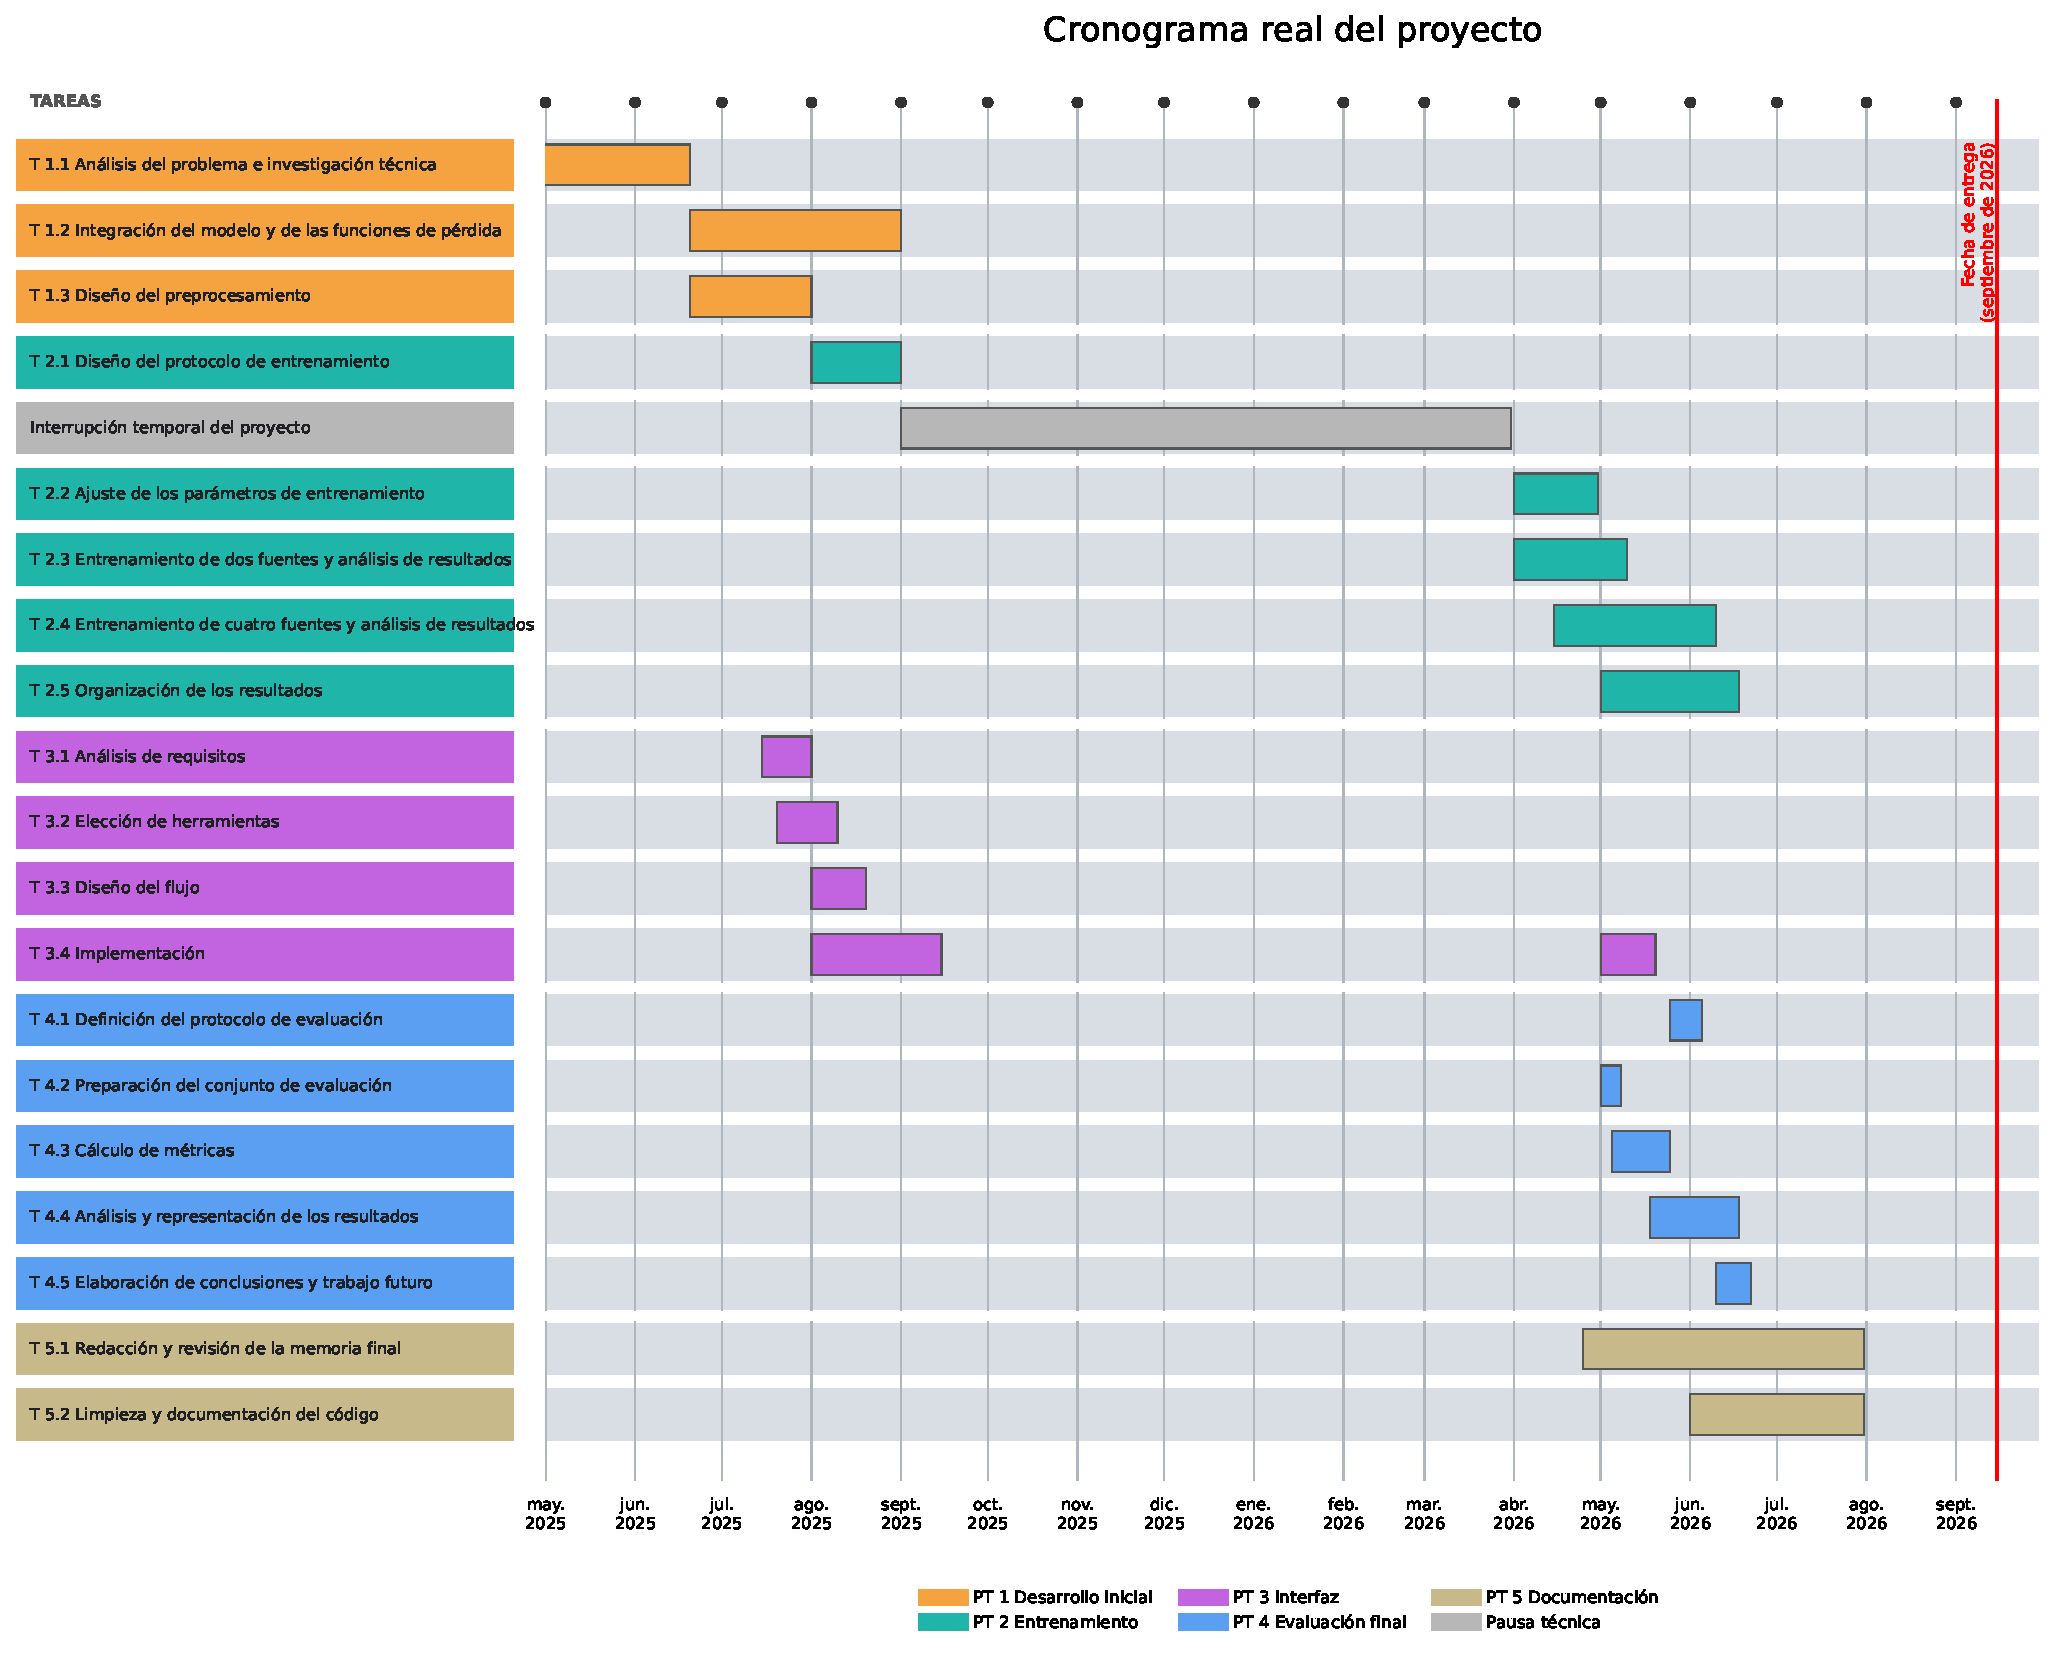
\includegraphics[
            width=1.25\textwidth,
            keepaspectratio
        ]{commons/cronograma_real_PT5_entrega_septiembre2026.pdf}%
    }
    \caption{Cronograma final del proyecto.}
    \label{fig:cronograma-final}
\end{figure}

Las incidencias que causaron este aumento en el tiempo dedicado se pueden resumir en los siguientes tres grupos:

\begin{itemize}
    \item \textbf{Incidencias por complejidad de la implementación:} 
    
    Errores en la implementación de carga de puntos de guardado y la implementación en el entrenamiento, y dimensiones en los valores calculados causaron gran impacto en las tareas 1.2,1.3 y 2.1.
    
    \item \textbf{Incidencias en el entrenamiento:} 
    
    Errores de parámetros, carga de datos y de modelos y de despliegue se terminaron por realizar tres tandas diferentes de entrenamientos, lo que causó gran impacto en las tareas 2.1,2.2,2.3 y 2.4.
    
    \item \textbf{Incidencias por coste computacional:} 
    
    Entrenar todas las funciones de pérdida resultó bastante más costoso de lo previsto inicialmente y causó gran impacto en las tareas 2.3 y 2.4.
\end{itemize}


Para resolver las desviaciones detectadas se aplicaron varias medidas correctoras:

\begin{itemize}
    \item Inferencia de la arquitectura del modelo a partir del \textit{state\_dict} del \textit{checkpoint}.
    \item Restauración de un método \textit{forward} coherente con el utilizado durante el entrenamiento.
    \item Unificación de la función \textit{run\_inference} para evaluación y despliegue.
    \item Creación de un conjunto de test fijo denominado \textit{representative\_test}.
    \item Incorporación de un \textit{baseline} de mezcla para validar los modelos frente a una solución trivial.
    \item Reentrenamiento mediante la versión V3 del protocolo experimental.
    \item Separación entre pérdidas principales, experimentales y avanzadas.
\end{itemize}

Aunque estas medidas provocaron un retraso respecto a la planificación inicial, permitieron establecer un proceso de evaluación más sólido obteniendo así mejores resultados. De este modo, se evitó seleccionar modelos únicamente por generar archivos de salida y se priorizó la obtención de resultados comparables, trazables y evaluables frente a un criterio común.

Siendo parte del proceso de la validación experimental, las incidencias ocurridas permitieron detectar y corregir errores que afectaban a la validez de los resultados
